\documentclass{article}

%% The graphicx and color packages should give you all the color,
%% figure inclusion, and text/figure resizing capabilities you need.
\usepackage{graphicx}
\usepackage[dvipsnames]{xcolor}
\usepackage{tikz,tikzsettings,bm}
\usepackage{almostfull}

\definecolor{pblue}{HTML}{1F77B4}
\definecolor{pgold}{HTML}{FF7f0E}
\definecolor{pgreen}{HTML}{2CA02C}
\definecolor{pred}{HTML}{D62728}
\definecolor{ppurple}{HTML}{9467BD}
\definecolor{ppink}{HTML}{E377C2}
\definecolor{pyellow}{HTML}{BCBD22}
\definecolor{pcyan}{HTML}{17BECF}

\usepackage{authblk}

%% You should not need more than this for fancy math.
\usepackage{amsmath}   % Extra math commands and environments from the AMS
\usepackage{amssymb}   % Special symbols from the AMS
\usepackage{amsthm}    % Enhanced theorem and proof environments from the AMS
\usepackage{latexsym}  % A few extra LaTeX symbols

\usepackage{lucidbry}
\input{stanacce}
\renewcommand{\baselinestretch}{1.0666}

%% The URL package is handy for typesetting URLs.  It does not define
%% an \email command because so many document styles already do that.
%% So we define one here that uses a typewriter font.
\usepackage{url}
%\DeclareRobustCommand{\email}{\begingroup \urlstyle{tt}\Url}
\providecommand{\email}{}
\renewcommand{\email}[1]{\texttt{#1}}

%% This provides various customized verbatim commands and
%% environments.  You probably don't need it.
\usepackage{fancyvrb}
\DefineShortVerb{\|}
\VerbatimFootnotes
\DefineVerbatimEnvironment{code}{Verbatim}{%
  frame=single,
  framesep=1em,
  xleftmargin=1em,
  xrightmargin=1em,
  samepage=true,
  fontsize=\footnotesize}
\usepackage{upquote}

%% Your document may require a different bibliography style.  I've
%% come to prefer Author (YYYY) styles because it makes it easier for
%% a person who knows something about the literature to understand
%% what is being cited without having to skip to the list of
%% references.
\usepackage[authoryear,round,longnamesfirst]{natbib}

%% You won't normally need this definition in your documents, but it
%% is here so we can typeset the BibTeX logo correctly.
\makeatletter
\@ifundefined{BibTeX}
   {\def\BibTeX{{\rmfamily B\kern-.05em%
    \textsc{i\kern-.025em b}\kern-.08em%
    T\kern-.1667em\lower.7ex\hbox{E}\kern-.125emX}}}{}

\def\blfootnote{\xdef\@thefnmark{}\@footnotetext}
\makeatother

%% Allow more of the pages to be occupied by graphs.  These parameters
%% are described in section c.9.1 of the LaTeXbook.  Your document may
%% not benefit from these parameters (it could make things worse) so
%% you should only change these from the defaults if you need to.
\setcounter{topnumber}{2}              %% 2
\setcounter{bottomnumber}{1}           %% 1
\setcounter{totalnumber}{3}            %% 3
\renewcommand{\topfraction}{0.9}       %% 0.7
\renewcommand{\bottomfraction}{0.9}    %% 0.3
\renewcommand{\textfraction}{0.1}      %% 0.2
\renewcommand{\floatpagefraction}{.7}  %% 0.5
\newlength{\graphwidth}
\setlength{\graphwidth}{0.8\columnwidth}

\usepackage{subfiles}

\graphicspath{{./}{./figures/}{./figures/paper/}}

\newcommand{\Is}{\bm{\mathrm{I}}} % Resources.
\newcommand{\Js}{\bm{\mathrm{J}}} % Units.
\newcommand{\Ks}{\bm{\mathrm{K}}} % Resources.
\newcommand{\Ms}{\bm{\mathrm{M}}} % Transition catalog.
\newcommand{\Ns}{\bm{\mathrm{N}}} % Transition counter.


\title{Data-based completion of grey-box models with neural networks}
\author{Pratyush Kumar}
\date{\today}

\begin{document}

\maketitle

\section{Process modeling}
Consider a nonlinear plant evolving in continuous time as
\begin{align*}
  \dot x &= f_p(x, u) \\
  y &= h_p(x)
\end{align*}
in which $x$ is the plant state (vector), $u$ is the manipulated control input,
and $y$ is the measurement. Assume that we don't have any 
disturbances/measurement and process noise 
for now, and we'll add those after we 
understand the issues in the nominal case.

\subsection{Completion of the u-y model}
We assume that grey-box modeling is performed 
for the plant, and we wish to augment the grey-box model with neural networks
for improvement in the accuracy of the model. From first-principles modeling, 
we have the following grey-box model in continuous time
\begin{align*}
  \dot{x}_g &= f_g(x_g, u) \\
  y &= h_g(x_g)
\end{align*}

in which $x_g$ are the grey-box states, which are some subset 
of the plant states (denote $x_g = Gx$) chosen to 
be modeled. The dynamics of these grey-box states 
potentially have some missing terms 
in their ODEs.
For observable nonlinear systems, 
we can construct the original plant state
using a history of measurements and control inputs.
Denote this history as 
\begin{align*}
  \mathbf{y}_{k:k-N} &= [y(k)', y(k-\Delta)', ..., y(k-N\Delta)']' \\
  \mathbf{u}_{k-1:k-N} &= [u(k-1)', u(k-2)', ..., u(k-N\Delta)']'
\end{align*}

in which $\Delta$ is the sample 
time between two consecutive
prediction instants of the desired discrete time 
model to be used in MPC. There exists a $\phi(\cdot)$ 
and a number of delay 
time steps $N$, such that the plant state
at a given time can be written as
$x(k) = \phi(\mathbf{y}_{k:k-N}, \mathbf{u}_{k-1:k-N})$.

We augment the grey-box model using 
neural networks as follows -
\begin{align*}
\dot x_g &= f_g(x_g, u) + 
f_{NN}(\mathbf{y}_{k:k-N}, \mathbf{u}_{k:k-N})\\
y &= h_g(x_g) + h_{NN}(\mathbf{y}_{k:k-N}, \mathbf{u}_{k-1:k-N})
\end{align*}
in which $f_{NN}(\cdot)$ and $h_{NN}(\cdot)$
are standard feedforward neural networks. We add the current 
control $u(k)$ as an input to the network $f_{NN}(\cdot)$ because 
there may be a mismatch in the actuator to the grey-box dynamics
as well.

It is expected that the functions $f_{NN}(\cdot)$ 
and $h_{NN}(\cdot)$ approximate
the following differences between the true grey-box state dynamics
and true measurement function with what is modeled.
\begin{align*}
  f_{NN}(\mathbf{y}_{k:k-N}, \mathbf{u}_{k:k-N}) &\approx 
      Gf_p(\phi(\mathbf{y}_{k:k-N}, \mathbf{u}_{k-1:k-N}), u) - f_g(x_g, u) = 
      Gf_p(x, u) - f_g(x_g, u) \\
      h_{NN}(\mathbf{y}_{k:k-N}, \mathbf{u}_{k-1:k-N}) &\approx 
      h_p(\phi(\mathbf{y}_{k:k-N}, \mathbf{u}_{k-1:k-N})) - h_g(x_g) = 
      h_p(x) - h_g(x_g) 
\end{align*}  

\subsection{Conversion to discrete time and training}
We note that the network $f_{NN}(\cdot)$ is an addition 
to the grey-box dynamics in continuous time, whereas 
$h_{NN}(\cdot)$ is an addition directly to the 
measurement function. The Runge-Kutta-4 (RK4) method 
is used for the discretization as follows

\begin{align*}
  k_1 &= f_g(x_g(k), u(k)) + f_{NN}(\mathbf{y}_{k:k-N}, \mathbf{u}_{k:k-N}) \\
  k_2 &= f_g(x_g(k) + (\Delta/2)k_1, u(k)) + 
         f_{NN}(\mathbf{y}_{k+0.5:k-N+0.5}, 
                \mathbf{u}_{k+0.5:k-N+0.5})\\
  k_3 &= f_g(x_g(k) + (\Delta/2)k_2, u(k)) + 
                f_{NN}(\mathbf{y}_{k+0.5:k-N+0.5}, 
                      \mathbf{y}_{k+0.5:k-N+0.5})\\
  k_4 &= f_g(x_g(k) + \Delta k_3, u(k)) + 
                       f_{NN}(\mathbf{y}_{k+1:k-N+1}, 
                              \mathbf{u}_{k+1:k-N+1})\\
  x_g(k+\Delta) &= x_g(k) + (\Delta/6)(k_1 + 2k_2 + 2k_3 + k_4) \\
  \hat{y}(k+\Delta) &= h_g(x_g(k+\Delta)) + h_{NN}(\mathbf{y}_{k+\Delta:k-N+\Delta}, 
                                     \mathbf{u}_{k-1+\Delta:k-N+\Delta})
\end{align*}
in which the sequences $\mathbf{y}_{k+0.5:k-N+0.5}$ 
and $\mathbf{u}_{k+0.5:k-N+0.5}$ are defined as 
\begin{align*}
  \mathbf{y}_{k+0.5:k-N+0.5} &= 
    [y(k + \Delta/2)', y(k-\Delta/2)', ..., y(k-N\Delta + \Delta/2)']' \\
  \mathbf{u}_{k+0.5:k-N+0.5} &= 
  [u(k + \Delta/2)', u(k-\Delta/2)', ..., u(k-N\Delta + \Delta/2)']' 
\end{align*}
We assume a zero order hold on the control inputs between two consecutive 
MPC execution instants, such that $u(k + \Delta/2) = u(k)$. To get the 
measurements between two sample instants ($y(k + \Delta/2)$) for 
the RK4 predictions, a linear interpolation can be used 
or we can assume that additional 
measurements from the plant are available 
between two MPC execution instants as well.

The following optimization problem is solved to compute 
the weights in the neural networks 
\begin{align*}
 \underset{W_{fi}, b_{fi}, W_{hi}, b_{hi}}{\textnormal{min}} \sum_{i=0}^{N_s-1} 
 \dfrac{1}{2}(\hat{y}(i) - y(i))^2
\end{align*}
in which ($W_{fi}, b_{fi}, W_{hi}, b_{hi}$) are the weights in the 
two neural networks ($f_{NN}(\cdot)$ and $h_{NN}(\cdot)$), 
$\hat{y}$ are predictions of the augmented model, and $y$
are the measurements from the plant.
Note that this optimization requires an estimate 
of the initial grey-box state. We assume that 
before the open-loop system identification experiment 
performed for data collection, 
the plant is being operated at some 
steady-state such that input to output
responses of the plant and grey-box model are aligned with 
the use of an integrating disturbance model. We can use 
the grey-box state at that steady state as the initial condition 
for the above multi-step-ahead prediction-error
optimization.

\subsection{Simple example}

Consider the following plant, model,
and the expected function to be approximated 
with a neural network.

\textbf{Plant --}
\begin{align*}
  \dfrac{dC_A}{dt} &= \dfrac{C_{A0} - C_A}{\tau} - k_1C_A\\
  \dfrac{dC_B}{dt} &= k_1C_A - k_2C_B + k_3C_C- \dfrac{C_B}{\tau}\\
  \dfrac{dC_C}{dt} &= k_2C_B - k_3C_C - \dfrac{C_C}{\tau}
\end{align*}
These ODEs represent the dynamics of the reaction system
$A \rightarrow B \rightleftharpoons C$ in a CSTR with constant 
height and temperature. The control input is $u = C_{A0}$,
the states are $x = [C_A, C_B, C_C]'$, 
and the measurements are $y = [C_A, C_B]'$. The plant model 
is observable with these choices of the measurements and dynamics.

\textbf{Model --}
\begin{align*}
  \dfrac{dC_A}{dt} &= \dfrac{C_{A0} - C_A}{\tau} - k_1C_A\\
  \dfrac{dC_B}{dt} &= k_1C_A - \dfrac{C_B}{\tau}
\end{align*}
i.e, we assume that we don't know about the second reaction while 
performing grey-box modeling. Assume the following 
parameter choices $k_1 = 1 \ \textnormal{m}^3/\textnormal{min}, 
\ k_2 = 10^{-2} \ \textnormal{m}^3/\textnormal{min}
\ k_3 = 10^{-3} \ \textnormal{m}^3/\textnormal{min}$, 
and $\tau = 20 \ \textnormal{min}$. 

Since the measurements are a simple linear function 
of the grey-box and plant states, we use only one network to 
augment the grey-box dynamics. The expected function 
to be approximated with a neural network is
\begin{align}
  f_{NN}(\mathbf{y}_{k:k-N}, \mathbf{u}_{k-1:k-N}) \approx (e^{A\Delta})^N
  \mathcal{O}(C, e^{A\Delta})^{\dagger}
\end{align}

 

\begin{figure}
  \centering
  \includegraphics[page=2, width=\textwidth]{tworeac_plots.pdf}
\end{figure}

%\textbf{Need to discuss the following issues:}
%\begin{itemize}
%  \item What are the example problems/applications 
%  where both kind of modeling 
%  strategies make sense, and where should we start.
%  Reproduce results from the Kevrekidis paper with measurement 
%  noise?
%  \item The model training step will be the optimization of 
%  the following multi-step-ahead prediction-error
%  \begin{equation*}
%    \underset{W_i, b_i}{\textnormal{min}} \sum_{k=0}^{t-1} (\hat{y}(k) - y(k))^2
%  \end{equation*}
%  in which ($W_i, b_i$) are the weights of the NN. This optimization 
%  is for one ID experiment, and requires an initial grey-box 
%  state $x_g(0)$ to make the forecast. If we have data 
%  for multiple ID experiments, we'll need initial states for 
%  all the ID experiments. In theory, we can add the initial 
%  states as decision variables in the optimization, but 
%  unfortunately tensorflow 
%  does not has a mechanism to do this.
%\end{itemize}

%\subsection{Adding feedforward disturbance forecasts}
%In this class of problems, we assume that we have a pretty 
%good u-y model from first-principles knowledge, and we'll use 
%neural networks to make feedforward disturbance forecasts
%for use in online MPC. HVAC is a pretty good application.

%\section{Optimization in MPC with neural networks as model}
%This is probably a late fall quarter or a winter break project. \\
%a) Try Casadi/MPC tools. 
%If tanh is the activation function (optimization is smooth),
%this should be fine. \\
%b) Try a global optimization solver. \\
%c) Train another NN with solutions from a global optimization solver.

\end{document}
